\section{Regimes}
\label{s:regimes}

In this section we discuss the various limits of
the expression describing the Hanle precession curve.
First, we show that the commonly used results for zero magnetic field
and tunneling contacts are correctly reproduced.
Next, we discuss regimes where appropriate scaling will give non-unique Hanle fits.
In the following, we mostly consider the case $r = r_0 = r_L$ of similar contacts.

In the limit of tunneling contacts, $R_C^0, R_C^L ≫ R_F$.
Putting $r_0, r_L → ∞$ gives $p_1 p_2 → \left( P_Σ^L \right)^2$ and
\begin{equation}
  f^∞ = \re{\frac{e^{- \left( L / λ \right) \sqrt{1 + i ω τ}}}{2 \sqrt{1 + i ω τ}}} ,
\end{equation}
which is of the same form as found in appendix B of
\cite{PhysRevB.37.5312}
(we will denote this limit with the superscript $∞$).
Fitting with this expression was found to give results equivalent
to fitting with the Hanle equation
\begin{equation}
  \label{eq:hanle_integral}
  \rNL^± = ± \sNL ∫_0^∞ \frac{e^{-t / τ}}{\sqrt{4 π D t}}
             \exp{\left[- \frac{L^2}{4 D t} \right]} \cos{ω t} \: dt .
\end{equation}
The agreement is expected as an explicit integration of \cref{eq:hanle_integral}
yields the same analytic expression provided $\sNL = {p_1 p_2 D} / {W σ_G}$.
In the additional limit of zero magnetic field,
\begin{equation}
  Δ \rNL = \left( P_Σ^L \right)^2 R_N e^{- L / λ} ,
\end{equation}
which agrees with eq. (6) in
\cite{PhysRevB.67.052409}.

Let $f_0$ denote $f$ at zero magnetic field,
\begin{equation}
  f_0 = \left[ 2 \left( 1 + λ / r \right) e^{L / λ} + \left( λ / r \right)^2 \sinh{L / λ} \right]^{-1} ,
\end{equation}
which agrees with eq. (3) in
\cite{PhysRevB.80.214427}.

To further explore the nature of the Hanle curves,
we exploit the fact that it only depends on
the dimensionless ratios $r / λ$, $L / λ$, and $ω τ$.
The only other parameter of the conducting channel that enters the expression
is the overall scale $λ$ in $R_N$.
The expression $f$ contains three terms
which are of zeroth, first, and second order in $λ / r$.
Thus, as the contact resistance decreases,
one goes from a device dominated by the first term to one dominated by the last.
But precisely how this comes about depends on the value of $ω τ$.

For infinite contact resistance, it was pointed out that any rescaling
of $g$, $τ$ and $D$ that leaves $λ$ and $ω τ$ unchanged
leads to the same Hanle precession curves
\cite{Swartz2013}.
Our result shows that the same is also true
when the contact resistance is taken into account.
In numerical simulations, interesting features where observed
when $L / λ ≪ 1$ and $r / λ ≪ 1$
\cite{PhysRevB.86.235408}.

To compare across regimes, we first normalize the data to its value at zero magnetic field.
In devices where $λ / r ≫ 1$, the normalization factor is
\begin{equation}
  f_0 = \frac{2 e^{- L / λ}}{\left( λ / r \right)^2} .
\end{equation}
In this regime, if $D$ is not very different from the infinite contact resistance value,
then the lifetime can be large, i.e., $τ ≫ \SI{1}{\nano \second}$.
As one tunes the magnetic field $\sqrt{ω τ} ≫ 1$, for small values of the field,
and for much of the curve, we can approximate $1 + i ω τ ≈ i ω τ$.
An interesting consequence of this is that the zero of the Hanle precession curve
becomes independent of the scattering time.
Note that the product
\begin{equation}
   \frac{L}{λ} \sqrt{ω τ} = L \sqrt{\frac{D}{ω}} ,
\end{equation}
which appears in the exponential and oscillating factors below,
is independent of the lifetime.
As one further tunes the magnetic field, the Hanle curve is given by
\begin{equation}
  \label{eq:regime.1.f}
  f = \frac{\sqrt{ω τ}}{\left( λ / r \right)^2}
      e^{- \left( L / λ \right) \sqrt{ω τ / 2}}
      \sin{\left[ \frac{L}{λ} \sqrt{\frac{ω τ}{2}} + \frac{π}{4} \right]} ,
\end{equation}
as long as $λ / r ≫ \sqrt{ω τ} ≫ 1$.
In this limit, the nonlocal resistance scales as
\begin{equation}
  \label{eq:regime.1.nonlocal_resistance}
  Δ \rNL ∝ \frac{λ \sqrt{ω τ}}{\left( λ / r \right)^2} = r^2 \sqrt{\frac{ω}{D}} ,
\end{equation}
and the normalized nonlocal resistance as
\begin{equation}
  f / f_0 ∝ \sqrt{ω τ} .
\end{equation}

On further increasing the field,
$\sqrt{ω τ} ≫ λ / r ≫ 1$, we get
\begin{equation}
  \label{eq:regime.2.f}
  f = \frac{1}{2 \sqrt{ω τ}}
      e^{- \left( L / λ \right) \sqrt{ω τ / 2}}
      \cos{\left[ \frac{L}{λ} \sqrt{\frac{ω τ}{2}} + \frac{π}{4} \right]} .
\end{equation}
In this limit, the nonlocal resistance scales as
\begin{equation}
  \label{eq:regime.2.nonlocal_resistance}
  Δ \rNL ∝ \frac{λ}{\sqrt{ω τ}} = \sqrt{\frac{D}{ω}} ,
\end{equation}
and the normalized nonlocal resistance as
\begin{equation}
  \label{eq:regime.2.ratio}
  f / f_0 ∝ \frac{\left( λ / r \right)^2}{\sqrt{ω τ}} = D \sqrt{\frac{τ}{ω r^4}} .
\end{equation}

In the limits of \cref{eq:regime.1.f,eq:regime.2.f},
the zeros of the Hanle fit are independent of the lifetime
and are determined by $D$ though the condition
\begin{equation}
  L \sqrt{\frac{D}{2 ω}} + \frac{π}{4} = \frac{n π}{2} ,
\end{equation}
where $n = 0$ for \cref{eq:regime.1.f} and $n = 1$ for \cref{eq:regime.2.f}.

\begin{figure}[!b]
  \caption{
    Data in figure 4 (d) from \cite{PhysRevLett.105.167202}
    fit to \cref{eq:nonlocal_resistance}
    with the same values as in
    \cref{fig:nonlocal_resistance.difference} (d).
    Fits with lifetimes that differ by four orders of magnitude
    were obtained by using different starting values for $τ$.
    These fits are otherwise similar with the exception of the lifetime,
    demonstrating the $τ$-independent scaling in \cref{eq:regime.1.nonlocal_resistance}.
    The $χ^2$ for \cref{fig:nonlocal_resistance.difference} (d)
    is \SI{2}{\percent} less than the $χ^2$ for
    \cref{fig:nonlocal_resistance.large_lifetime}.
  }
  \label{fig:nonlocal_resistance.large_lifetime}
  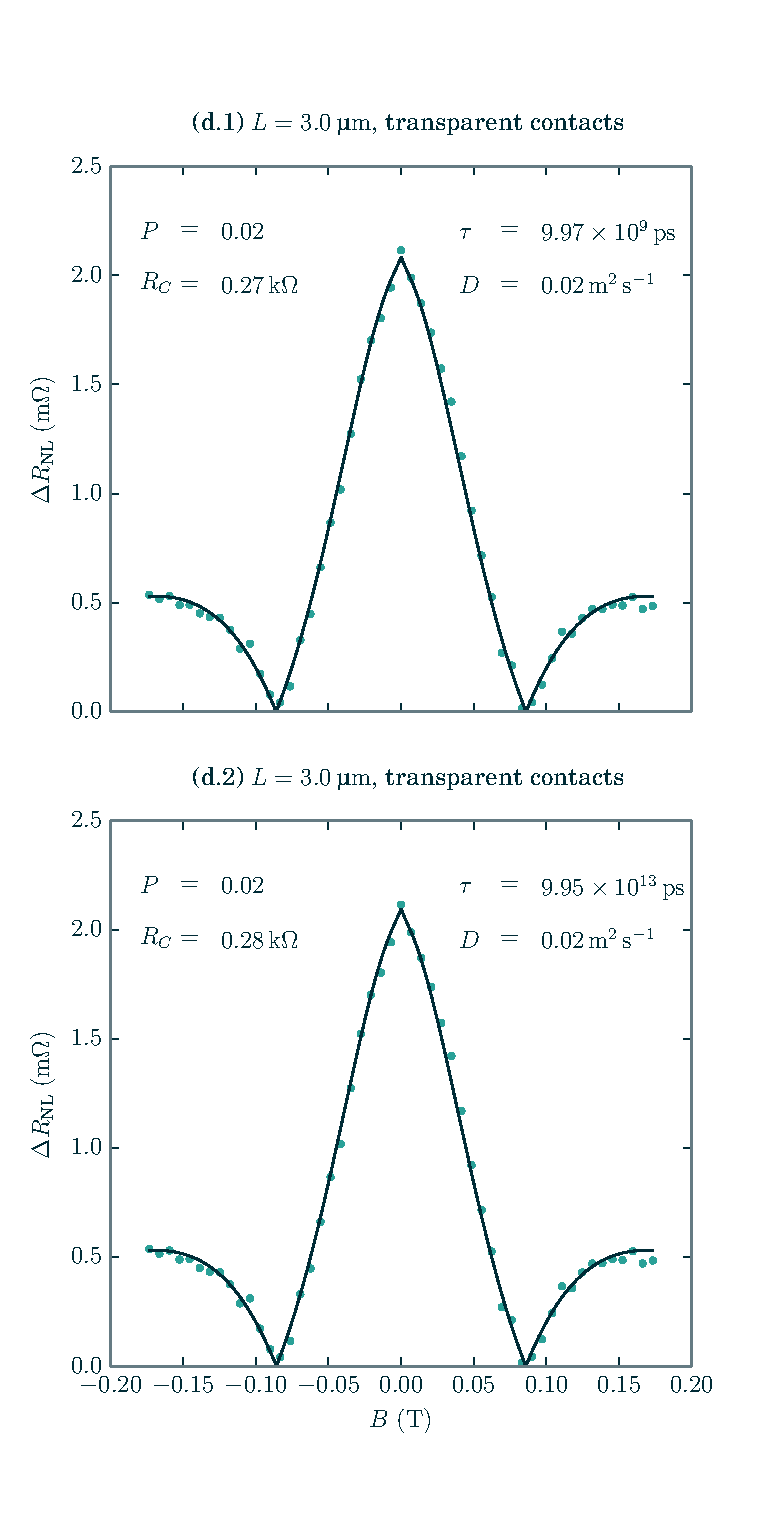
\includegraphics[width=\columnwidth]{figures/plot_large_lifetime}
\end{figure}

Note that fitting is insensitive to $τ$ in the limit of
\cref{eq:regime.1.nonlocal_resistance}
or \cref{eq:regime.2.nonlocal_resistance}.
As an example of this,
\cref{fig:nonlocal_resistance.large_lifetime} shows nearly identical fits
with lifetimes that differ by four orders of magnitude.
These fits were obtained by choosing large starting values for $τ$.
For \cref{fig:nonlocal_resistance.difference} (d)
and \cref{fig:nonlocal_resistance.large_lifetime},
$χ^2 ∼ \SI{7e-8}{}$, but the $χ^2$ for
\cref{fig:nonlocal_resistance.difference} (d)
is \SI{2}{\percent} less than the $χ^2$ for
\cref{fig:nonlocal_resistance.large_lifetime}.
In \cref{fig:nonlocal_resistance.difference} (d),
$λ / r ≫ \sqrt{ω τ}$ and $ω τ ∼ 1$ for most of the curve,
so the approximation $1 + i ω τ ≈ i ω τ$ does not hold.
However, \cref{fig:nonlocal_resistance.large_lifetime}
is in the limit of \cref{eq:regime.1.nonlocal_resistance}
for all points (save the origin).
Thus, in limit of small $r$, the fitted value of $τ$ is unreliable
unless one carefully controls the fitting procedure.

The evolution of the expression for the Hanle curve
is an interesting insight into the behavior of the device.
Fitting data on devices with small contact resistances
with the functional form applicable to infinite contact resistance
yields unreliable parameters.
In particular, they were numerically shown to severely underestimate the spin lifetime
\cite{PhysRevB.86.235408}.

Further analytic progress can be made if one assumes that
lifetimes as estimated with infinite contact resistance are long
enough that the approximation of $\sqrt{ω τ} ≫ λ / r ≫ 1$
is still valid for much of the data being analyzed.
For this case, at infinite contact resistance,
the normalized nonlocal resistance is given by
\begin{equation}
  \frac{f^∞}{f^∞_0} = \frac{1}{ \sqrt{ω τ}}
                      e^{- \left( L / λ \right) \sqrt{ω τ / 2}}
                      \cos{\left[ \frac{L}{λ} \sqrt{\frac{ω τ}{2}} + \frac{π}{4} \right]} .
\end{equation}
Provided $D$ remains constant,
this will yield the same curve with finite contact resistance if
\begin{equation}
  \label{eq:lifetime_scale.infinity}
  \frac{1}{τ^∞} = D^2 \frac{τ}{r^4} .
\end{equation}
In other words, if we fix $τ$ and ask what happens to the fitted value
assuming infinite contact resistance as a function of decreasing $r$,
\cref{eq:lifetime_scale.infinity} shows that it will decrease as well.
For $D$ fixed, $τ^∞ ∝ r^4$.
While the general trend is consistent with
\cite{PhysRevB.86.235408},
the quantitative agreement is limited by
the approximations made for analytic convenience.
